\documentclass{article}
\usepackage[utf8]{inputenc}
\usepackage[spanish]{babel}
\usepackage{bytefield}
\usepackage{amsmath}
\usepackage{array}
\usepackage{booktabs}
\usepackage{graphicx}
\usepackage{longtable}
\usepackage{hyperref}
\usepackage{makecell}
\usepackage{float}

\title{Trabajo Práctico
Administración de Redes Locales}
\author{Ignacio Mastrangelo, Renzo Portela, Luca Bogado}
\date{28 de marzo de 2025}

\begin{document}

\maketitle

\subsection{GitHub LINK:} 

\section*{Direcciones}
IPV6 autoconfigurada LLA PCO: FE80::2EO:F9FF:FE98:8A07

Dirección mac fastethernet 0 PCO : 00EO.F998.8A07

\section*{Relación entre IPv6 y MAC}
La relación entre la dirección IPv6 autoconfigurada (LLA, Link-Local Address) y la dirección MAC en tu ejemplo se explica mediante el algoritmo EUI-64, que convierte una MAC de 48 bits en una Interface ID de 64 bits para IPv6.

1. \textbf{Dividir la MAC en dos partes (24 bits c/u):}

   [00EO.F9] (OUI)  
   [98.8A.07] (NIC specific).

2. \textbf{Insertar} FFFF en el medio:

   * MAC original: 00:EO:F9:98:8A:07
   * MAC modificada: 00:EO:F9:FF:FE:98:8A:07

   (Se añade  FFFE  entre los bytes 3 y 4).

3. \textbf{Invertir el bit U/L (7º bit del primer byte):}

   * Primer byte original (hex): 00 → binario: 00000000
   * 7º bit (U/L): 0 (local) → se cambia a 1 (global):

    00000000 → 00100000 (hex: 20 ).

   * Resultado: El primer byte cambia de 00 a 20 .

4. \textbf{Interface ID final (64 bits):}

   * MAC modificada con bit U/L invertido: 20:EO:F9:FF:FE:98:8A:07
   * En IPv6: 20EO:F9FF:FE98:8A07 (se omite : cada 2 bytes).

\section*{IPv6 Link-Local completa}
5. \textbf{IPv6 Link-Local completa:}

- Prefijo Link-Local:  FE80::/64
- Interface ID:  20E0:F9FF:FE98:8A07
- \textbf{Dirección final:}  FE80::20E0:F9FF:FE98:8A07

\begin{figure}[h]
    \centering
    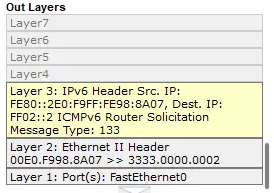
\includegraphics[width=0.8\textwidth]{imagen1.PNG}
    \caption{Descripción de la imagen}
    \label{fig:ejemplo}
\end{figure}


El mensaje \textbf{Router Solicitation (RS)} enviado por \textbf{PC0} utiliza el protocolo \textbf{ICMPv6} como parte del proceso \textbf{NDP (Neighbor Discovery Protocol)}.

\section*{Campos clave del mensaje Router Solicitation (RS):}
\begin{tabular}{|l|l|}
\hline
Campo & Valor/Descripción \\
\hline
IPv6 Source & FE80::[Interface\_ID]  (LLA de PCO, derivada de MAC vía EUI-64). \\
IPv6 Destination & FF02::2  (All-Routers multicast). \\
ICMPv6 Type & 133  (Router Solicitation). \\
Ethernet Dest MAC & 3333.0000.0002  (Multicast para routers). \\
Hop Limit & 255  (para validar que el mensaje es local) \\
\hline
\end{tabular}
Avanzamos hasta que PCO reciba el mensaje de respuesta:

\begin{figure}[h]
    \centering
    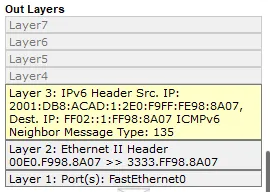
\includegraphics[width=0.8\textwidth]{imagen2.PNG}
    \caption{Descripción de la imagen}
    \label{fig:ejemplo}
\end{figure}

Vemos como ahora PC0 tiene una dirección GUA.
\begin{figure}[h]
    \centering
    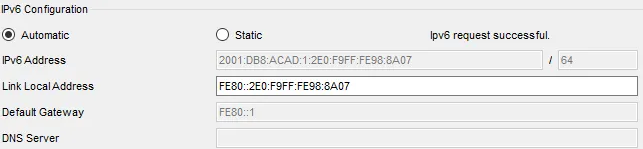
\includegraphics[width=0.8\textwidth]{imagen3.PNG}
    \caption{Descripción de la imagen}
    \label{fig:ejemplo}
\end{figure}


PCO obtiene su GUA ( 2001:DB8::2E0:F9FF:FE98:8A07 ) mediante SLAAC(1), usando el prefijo del RA y su Interface ID (EUI-64).

\textbf{SLAAC} (Stateless Address Autoconfiguration) es un mecanismo del protocolo IPv6 que permite a los dispositivos generar automáticamente sus propias direcciones Global Unicast Address (GUA) y Link-Local Address (LLA) sin necesidad de un servidor central como DHCPv6

\section*{2 Neighbor Discovery}
\subsection*{2.1 Local delivery}
\textbf{P1}

Los mensajes NDP (Neighbor Discovery Protocol) aparecen porque IPv6 no usa ARP (como en IPv4), sino NDP para resolver direcciones MAC. En este caso:\\
1- PCO quiere hacer ping a 2001:DB8:ACAD:1::B (PC1), pero no conoce su MAC.\\
2- Neighbor Solicitation (NS): PCO envía una solicitud para descubrir la MAC de ::B.\\
3- Neighbor Advertisement (NA): PC1 responde con su MAC.
\\

De los 13 paquetes son varios los tipos:\\
-ICMPv6 Echo Request/Reply (ping).\\
-NS/NA (resolución de MAC).\\
-Mensajes de multicast (como FF02::1:FF00:000B).

\textbf{P2}

Al abrir el primer mensaje en PCO, vemos como el tipo de mensaje es ICMPv6 Type 128, equivalente a un ping en IPv4 pero en IPv6.

\begin{tabular}{|l|}
\hline
Layer 3: IPv6 Header Src. IP:\\
 2001:DB8:ACAD:1::A, Dest. IP: \\
2001:DB8:ACAD:1::B ICMPv6 Echo\\
Message Type: 128 \\
\hline
\end{tabular}
\\

Al mirar el direccionamiento del paquete, notamos que en capa 2 PCO ya tenía en su tabla una dirección MAC que coincidía "The next-hop IP address is in the neighbor table. The ND Process sets the frame's destination MAC address to the one found in the table". Esto nos recorrobora que cuando un host ya tiene la MAC del destino en su tabla, omite el proceso de NDP y envía el frame directamente a la MAC unicast.

\subsection*{P3}
Al analizar los cambios en layer 2 y 3 de cada PDU, notamos que:

1. Capa de Red (Layer 3):

- \textbf{Dirección IPv6 de origen:} FE80:::(enlace local)
   → 2001:DBB:ACAD:::A (unicast global).

- \textbf{Dirección IPv6 de destino:} FF02:::(multicast)
   → 2001:DBB:ACAD:::B (unicast).

- \textbf{Tipo de mensaje ICMPv6:} 134 (Router Advertisement) → 128 (Echo Request).

2. Capa de Enlace (Layer 2):

- \textbf{MAC de origen:} 000D.BD9D.BC01 → 0090.2B89.2D86 .

- \textbf{MAC de destino:} 3333.0000.0001 (multicast) → 0090.0C58.E7DC (unicast).\\
En IPv6 cuando un host necesita descubrir la dirección MAC de otro dispositivo en su red local (similar al ARP en IPv4), el NDP (Neighbor Discovery Protocol). A diferencia de IPv4, que usa broadcast (FFFFFFFFFFFFFF ), IPv6 emplea multicast dirigido para mayor eficiencia, utilizando direcciones MAC especiales del tipo 3333.XXXX.XXXX . La dirección MAC 3333.XXXX.XXXX es fundamental en IPv6 para el descubrimiento de vecinos (NDP), permitiendo una resolución de direcciones más eficiente que el ARP de IPv4.



\begin{tabular}{|l|l|}
\hline
In Layers & Out Layers \\
\hline
Layer7 & Layer7 \\
Layer6 & Layer6 \\
Layer5 & Layer5 \\
Layer4 & Layer4 \\
Layer3 & Layer3 \\
\makecell[l]{Layer 2: Ethernet II Header \\ 000D.BD9D.8C01 \textgreater\textgreater 3333.0000.0001} & \makecell[l]{Layer 2: Ethernet II Header \\ 000D.BD9D.8C01 \textgreater\textgreater 3333.0000.0001} \\
Layer 1: Port GigabitEthernet0/1 & Layer 1: Port(s): FastEthernet0/1 FastEthernet0/2 \\
\hline
\end{tabular}

Al comparar ambos PDU notamos que las MAC de destino y origen se mantienen. El switch al recibir una mac multicast en su tabla, reenvía el paquete por todos los puertos menos por el que lo recibió. En conclusión, el switch modifica el camino de la trama (puertos de salida), pero no altera las direcciones L2.

\subsection*{P5}

\text 
Ethernet Destination Address: 3333.FF00.000B\\
Ethernet Source Address: 0090.0C5B.E7DC\\
IPv6 Source Address: 2001:DB8:ACAD:1::B\\
IPv6 Destination Addres: FF02::1:FF00:B\\

\subsection*{P6}
El motivo por el cual no hay información en Out Layers se explica en los puntos 4 al 7 del registro: \\
\hspace{1cm}-El paquete es un mensaje ICMPv6 Neighbor Solicitation (Tipo 135) que forma parte del protocolo NDP (Neighbor Discovery Protocol).\\
\hspace{1cm}-El punto 6 indica que "la dirección IPv6 objetivo de la Neighbor Solicitation no coincide con la dirección IPv6 del puerto receptor".\\
\hspace{1cm}-Como consecuencia de lo anterior, el proceso NDP decide descartar el paquete (punto 7).\\

\subsection*{P7}
Podemos afirmar que PCO tiene toda la información necesaria para
comunicarse con PC1 ya que Conoce la dirección IPv6 de PC1, Ha resuelto la
dirección MAC de PC1 (evidenciado por la presencia de la MAC destino en el
encabezado Ethernet) y El paquete ICMPv6 muestra que la comunicación está
activa.

\subsection*{P8}
Es un mensaje de tipo 129(echo), es decir que es un mensaje de respuesta y
que confirma que existe comunicación entre PCO y PC1.

\subsection*{P9}
No hubo ningun evento NPD ya que PKT conserva la caché de vecinos,
evitando tener que utilizar NPD. En otras palabras reutiliza la información
almacenada de procesos previos, para evitar el uso del NPD.

\section*{2.2 Non Local delivery}
\textbf{P1}

Reseteamos la simulacion\\


\vspace{2cm}

\textbf{P2}
\begin{figure}[h]
    \centering
    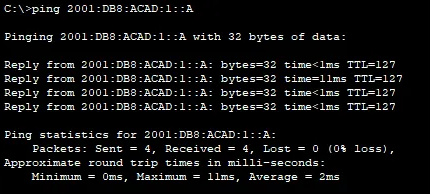
\includegraphics[width=0.8\textwidth]{imagen4.PNG}
    \caption{Descripción de la imagen}
    \label{fig:ejemplo}
\end{figure}



Realizo el ping entre PC2 y PC0

\subsection*{P3}
\begin{figure}[h]
    \centering
    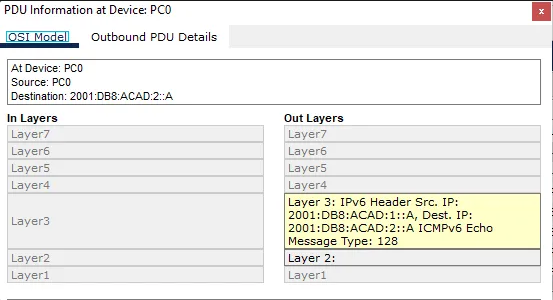
\includegraphics[width=0.8\textwidth]{imagen5.PNG}
    \caption{Observamos que carece de Layer 2 al hacer el ping entre estos PCs}
    \label{fig:ejemplo}
\end{figure}

\subsection*{P4}

\begin{figure}[H] 
    \centering
    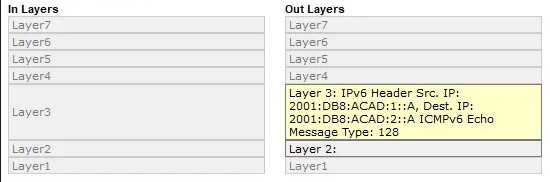
\includegraphics[width=0.8\textwidth]{imagen6.PNG}
    \caption{}
    \label{fig:ejemplo}
\end{figure}

Tipo de mensaje ND: ICMPv6 Neighbor Solicitation (NS) - Tipo 135

Dirección IPv6 de origen: FE80::290:2BFF:FE89:2D86 (link-local de PC0).

\subsection*{P5}
\begin{figure}[H] 
    \centering
    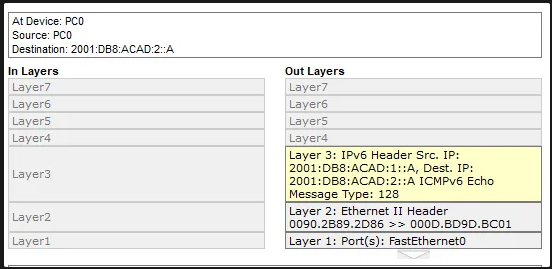
\includegraphics[width=0.8\textwidth]{imagen7.PNG}
    \caption{}
    \label{fig:ejemplo}
\end{figure}



Direcciones L2 encapsuladas:\\

**MAC origen:** 0090.2B89.2D86 (La MAC de PC0)\\
**MAC destino:** 000D.BD9D.BC01 (La MAC del puerto del router)\\

PC0 ya realizó una resolución de dirección L2 (con un Neighbor Solicitation previo) para obtener la MAC asociada a la IPv6 del host destino, en este caso descubre que la IPv6 de destino está en otra red, por lo que la MAC de destino es del router(la default gateway de PC0).

\subsection*{P6}
\begin{figure}[H] 
    \centering
    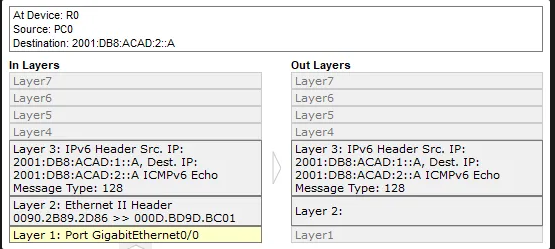
\includegraphics[width=0.8\textwidth]{imagen8.PNG}
    \caption{}
    \label{fig:ejemplo}
\end{figure}


El router R0 necesita enviar un ICMPv6 Neighbor Solicitation (Tipo 135) para descubrir la dirección MAC asociada a 2001:DBS:ACAD:2::A antes de reenviar el mensaje ICMPv6 Echo Request.\\

R0 no tiene la MAC destino en su caché de vecinos. Suponemos que el proximo paquete será de tipo NPD, ya que R0 necesita descubrir la MAC de destino.
\subsection*{P7}
\begin{figure}[H] 
    \centering
    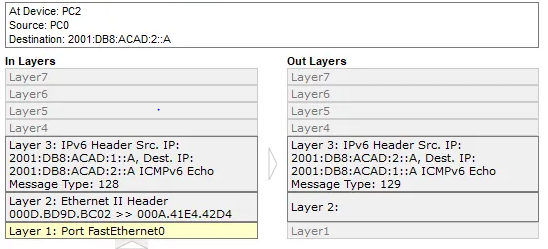
\includegraphics[width=0.8\textwidth]{imagen9.PNG}
    \caption{}
    \label{fig:ejemplo}
\end{figure}



Tipo de mensaje ICMPv6 saliente: Echo Reply (Tipo 129)\\

PC 2 no tiene la dirección MAC destino (si no está en la caché NDP de PC2). PC2 encontrar la MAC asociada a la IPv6 2001:DB8:ACAD:1::A por esto suponemos que tendremos una secuencia de paquetes NPD.

\
\subsection*{P8}
\begin{figure}[H] 
    \centering
    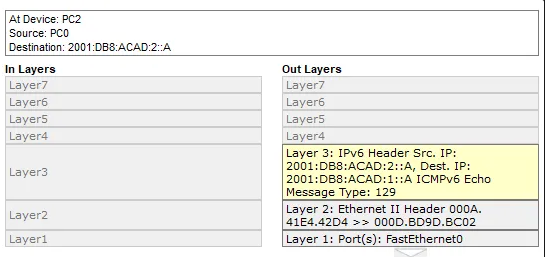
\includegraphics[width=0.8\textwidth]{imagen10.PNG}
    \caption{}
    \label{fig:ejemplo}
\end{figure}


Observamos que luego de todos los paquetes, se logra entender todas las direcciones en distintas Layers.

\subsection*{P9}
\begin{figure}[H] 
    \centering
    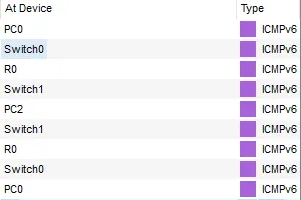
\includegraphics[width=0.8\textwidth]{imagen11.PNG}
    \caption{}
    \label{fig:ejemplo}
\end{figure}


No hubo eventos NDP porque las direcciones MAC ya estaban cacheadas. PC0 y R0 ya conocían las direcciones físicas necesarias, por lo que el ping se envió directamente sin necesidad de resolver direcciones.

MAC destino en PC2:

000D.BD9D.BC02	 Es la MAC de destino del router(default gateway de PC2)

GIGA0/1.

\subsection*{P10}
\section*{R0\#show ipv6 neighbors}
\begin{tabular}{|l|l|l|l|}
\hline
IPv6 Address & Age Link-layer Addr & State Interface \\
\hline
2001:DBB:ACAD:1::A & 1 0090.2B89.2D86 & REACH Gig0/0 \\
2001:DBB:ACAD:2::A & 1 000A.41E4.42D4 & REACH Gig0/1 \\
FE80::20A:41FF:FE84:42D4 & 1 000A.41E4.42D4 & REACH Gig0/1 \\
FE80::290:2BFF:FE89:2D86 & 1 0090.2B89.2D86 & REACH Gig0/0 \\
\hline
\end{tabular}

\subsection*{Número de direcciones en la lista:}
Aparecen 4 direcciones IPv6 en la tabla de vecinos de R0.

\subsection*{Dispositivos asociados:}
2001:DB8:ACAD:1:A → MAC  0090.2B89.2D86

2001:DB8:ACAD:2::A → MAC  000A.4IF4.42D4

Direcciones link-local:

FE80::290:2BFF:FE89:2D86 → Misma MAC  0090.2B89.2D86

FE80::20A:4IFF:FE84:42D4 → Misma MAC  000A.4IF4.42D4

¿Hay entrada para PC1?

No, no aparece ninguna entrada para PC1 en la lista.

La tabla solo muestra dispositivos conectados directamente a R0 (PC0 en Gig0/0 y PC2 en Gig0/1).

\subsection*{P11}
Tras el ping a PC1 desde R0: Observamos como ahora si PC1 tiene una entrada en la lista de neighbors de R0.

\begin{tabular}{|l|l|l|l|}
\hline
IPv6 Address & Age Link-layer Addr & State Interface \\
\hline
2001:DB8:ACAD:1::A & 1 0090.2B89.2D86 & REACH Gig0/0 \\
2001:DB8:ACAD:1::B & 0 0090.0C5B.F7DC & REACH Gig0/0 \\
2001:DB8:ACAD:2::A & 1 000A.41F4.42D4 & REACH Gig0/1 \\
FE80::20A:4IFF:FE84:42D4 & 1 000A.41F4.42D4 & REACH Gig0/1 \\
FE80::290:2BFF:FE89:2D86 & 1 0090.2B89.2D86 & REACH Gig0/0 \\
\hline
\end{tabular}

\section*{3 CONCLUSIONES}
1. ¿Que ventaja y desventajas plantea la autoconfiguración de IPv6?

Algunas ventajas que propone la autoconfiguración IPv6:

SLAAC simplifica la configuración de red porque los dispositivos pueden obtener automáticamente una dirección IPv6 usando el prefijo del router y su dirección MAC mediante el algoritmo EUI-64. Esto reduce la carga administrativa y evita la necesidad de configurar manualmente cada dispositivo. Esto elimina la dependencia de un servidor DHCP.

Algunas desventajas:

SLAAC no permite personalización avanzada, como asignar parámetros específicos (DNS, por ejemplo).Además encontramos problemas de privacidad porque la dirección MAC se incorpora en la dirección IPv6 mediante EUI-64, lo que podría exponer información del dispositivo.

2. ¿Que tipos de mensajes se utilizan en la configuración vs el descubrimiento y como se relacionan?

En IPv6, los procesos de configuración y descubrimiento de vecinos utilizan mensajes específicos del protocolo ICMPv6 que trabajan de forma coordinada. Los mensajes clave para la autoconfiguración son el Router Solicitation (RS) y Router Advertisement (RA).Estos dos mensajes se relacionan fuertemente ya que, un dipositivo envía un RS al grupo multicast del router y estos responden con un RA que incluye los parametros esenciales para la configuración.

Por otro lado el descubrimiento de vecinos emplea los mensajes NS (Neighbor Solicitation) y NA(Neighbor Advertisement).Cuando un host necesita comunicarse con otro en su misma red, primero envía un NS al grupo multicast solicitando la dirección MAC asociada a una IPv6 específica. El host destino responde con un NA que contiene su dirección MAC, completando así la resolución de direcciones

3. ¿Cuando requiere un dispositivo el proceso de detección de vecinos IPv6?

Un dispositivo requiere de el proceso de detección de vecinos en IPv6 (NDP) se activa cuando este necesita resolver la dirección MAC asociada a una IPv6 en la misma red (similar al ARP IPv4), descubrir routers locales para configurar direcciones automáticamente (SLAAC) para mantener la conectividad. También entra en juego cuando un router informa una mejor ruta mediante redireccionamiento. Este mecanismo es fundamental durante el inicio de interfaces IPv6, el envío de tráfico a nuevos destinos o la detección de cambios en la topología de red.

4. ¿Como ayuda un router a minimizar la cantidad de tráfico IPv6 Neighbor Discovery en una red?

Un router ayuda a minimizar la cantidad de tráfico IPv6 Neighbor Discovery (ND) en una red al actuar como intermediario para la comunicación entre dispositivos en diferentes subredes. Esto se ve reflejado cuando PC0 intenta comunicarse con otro en una red distinta (por ejemplo, PC2), el router (R0) maneja la resolución de direcciones MAC necesarias para el reenvío de paquetes. En lugar de generar múltiples mensajes ND en toda la red, el router utiliza su tabla de vecinos (cache NDP) para almacenar las direcciones MAC de los dispositivos conectados directamente a sus interfaces, como se observa en la tabla de vecinos de R0.

5. ¿Como minimiza IPv6 el impacto del proceso ND en los hosts de red?

IPv6 minimiza el impacto del proceso de Neighbor Discovery (ND) en los hosts de red mediante mecanismos más eficientes en comparación con IPv4, como el uso de direcciones multicast específicas en lugar de broadcast. Esto genera un tráfico mucho mas controlado.

6. ¿En que difiere el proceso de deteccion de vecinos cuando un host de destino esta en la misma LAN y cuando está en una LAN remota?

El proceso de detección de vecinos (ND) en IPv6 varía según si el host de destino está en la misma LAN o en una remota. En la misma LAN, el host origen envía un mensaje Neighbor Solicitation (NS) a una dirección multicast específica (FF02::1:FFXX:XXXX), dirigido solo a dispositivos con la IPv6 objetivo, y el destino responde directamente con un Neighbor Advertisement (NA), resolviendo la MAC sin intervención de routers.

En una LAN remota, el host origen no intenta resolver la MAC del destino final, sino que envía el tráfico a su gateway predeterminado (router) usando la MAC de este. El router luego gestiona la resolución en la red destino, enviando un NS si no tiene la MAC en cache. Así, IPv6 evita tráfico innecesario en redes remotas y optimiza el proceso mediante multicast dirigido en la LAN local.

\end{document}